%\chapter*{Введение}
%\addcontentsline{toc}{chapter}{Введение}

\newpage
\textbf{2 Проектирование БТС}
\refstepcounter{chapter}
\addcontentsline{toc}{chapter}{2 Проектно-конструкторская часть}
%\settocdepth{subsubsection}

\section{Разработка макета адаптера}
Позиционирование УЗ-датчика делится на два этапа: приблизительное размещение датчика в области исследования и более точная установка (выбор угла поворота и силы прижатия датчика). Для осуществления этих этапов необходимо разработать адаптер для крепления УЗ-датчика к конечному звену манипулятора, конструкция которого удовлетворяет следующим требованиям:

- возможность присоединения к конечному звену робота-манипулятора UR5e,

- обеспечение быстрого закрепления  и снятия ультразвукового датчика с помощью удобных для пользователя механизмов, 

- минимизация искажений измеренных сигналов на датчике силы, возникающих из-за сил тяжести, действующих на кабели устройства.

Исходя из геометрических параметров УЗ-датчика был спроектирован адаптер (рисунок 8а), состоящий из трех частей: основания (рисунок 8б), прижимной планки (рисунок 8в) и прижима провода (рисунок 8г).

Из-за криволинейной формы ручки датчика для надежности фиксации было выбрано винтовое соединение составных частей. 

Основание с помощью винтов прикручивается к конечному звену манипулятора, затем устанавливается УЗ-датчик и фиксируется прижимной планкой с помощью винтов. Для быстрого закрепления и снятия используются зажимные винты-барашки. Для обеспечения фиксации соединительного кабеля спроектирован прижим, который закрепляется на основании с помощью винтов со сферической головкой AS 1427H M4x16. 

\begin{figure}[H]
\begin{minipage}[h]{0.47\linewidth}
\center{\includegraphics[width=1\linewidth]{сборка.png}} a) \\
\end{minipage}
\hfill
\begin{minipage}[h]{0.47\linewidth}
\center{\includegraphics[width=1\linewidth]{основание.png}} \\б)
\end{minipage}
\vfill
\begin{minipage}[h]{0.47\linewidth}
\center{\includegraphics[width=1\linewidth]{планка.png}} в) \\
\end{minipage}
\hfill
\begin{minipage}[h]{0.47\linewidth}
\center{\includegraphics[width=1\linewidth]{прижим.png}} г) \\
\end{minipage}
\caption{3Д-модель макета адаптера для конечного звена манипулятора: a - адаптер в сборе; б - основание; в - планка прижимная; г - прижим провода}
\label{ris:experimentalcorrelationsignals}
\end{figure}

%Для данной конструкции выбрана однолистовая изогнутая пружина. Материал – АМг2М (сплав алюминия, легированного магнием и марганцем). Характеристики данной пружины следующие: 

%– давление (нагрузка на контакты) $P=0,4$ кг,

%– длина рабочей части пружины $L=30$ мм,

%– допускаемое напряжение на изгиб при переменной нагрузке $R_b=49$ кг/мм$^2$,

%– модуль упругости $E=7000$~кг/мм$^2$,

%– прогиб пружины $f=15$ мм. 


%Определим толщину пружины:\\
%\begin{equation}\label{tol}
%h=\frac{2\cdot L^2 \cdot R_b}{3 \cdot f \cdot E}.
%\end{equation}
%$h=0,28$ мм.

\section{Анализ технологичности конструкции макета адаптера}
Конструкция имеет простую компоновку и простое конструктивное решение, что не вызывает затруднений при сборке. В конструкции предусматриваются базовые детали, которые являются основой для расположения остальных составных частей узла. Масса всех деталей узла не превышает 0,5 кг. Можно легко производить замену деталей в процессе эксплуатации, что удешевляет ремонт. Конструкция сборочной единицы  обеспечивает возможность ее сборки из предварительно собранных составных частей.


Данное конструктивное решение позволяет выполнять все необходимые функции БТС и удовлетворяет всем требованиям для получения оптимального сигнала: обеспечивает точное позиционирование  спектрофотометрических датчиков на голове, не производит механическую нагрузку на исследуемую область, позволяет проводить измерения при движении пациента. Для улучшения конструкторской разработки можно увеличить количество каналов, что позволит проводить зондирование на разных расстояниях между источником и детектором.

\section{Прочностной расчет конструкции макета адаптера}
Для расчета конструкции на прочность в ПО Ansys смоделировано действие двух типов нагрузок (рисунок 2.7).
\begin{figure}[!h]
\begin{center}

\begin{minipage}[h]{0.45\linewidth}
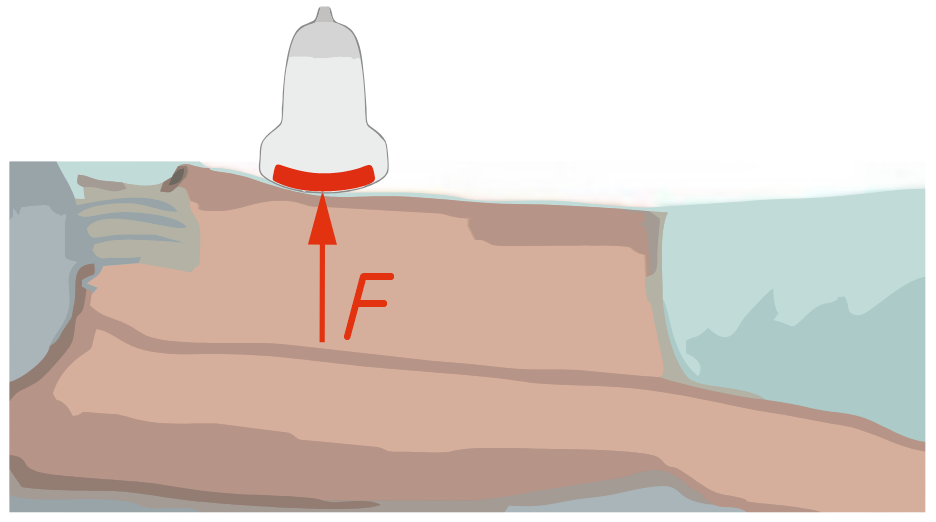
\includegraphics[width=\textwidth, keepaspectratio]{сила1}
\end{minipage}
%\hfill
\begin{minipage}[h]{0.45\linewidth}
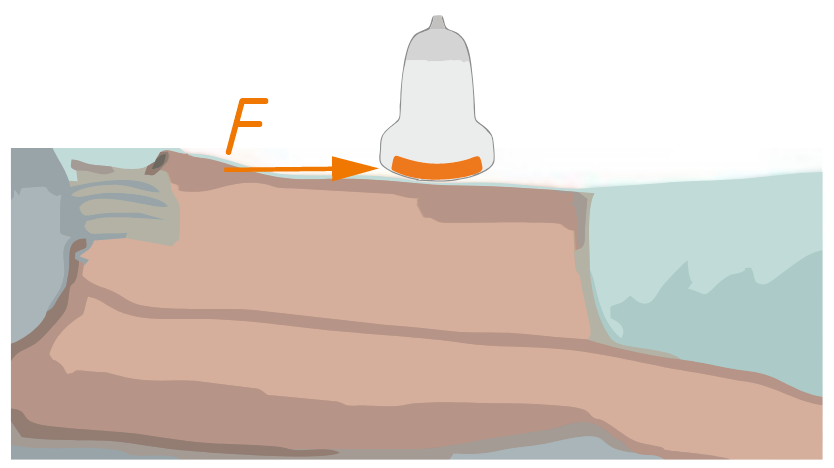
\includegraphics[width=\textwidth, keepaspectratio]{сила2}
\end{minipage}
\begin{minipage}[!h]{0.45\linewidth}
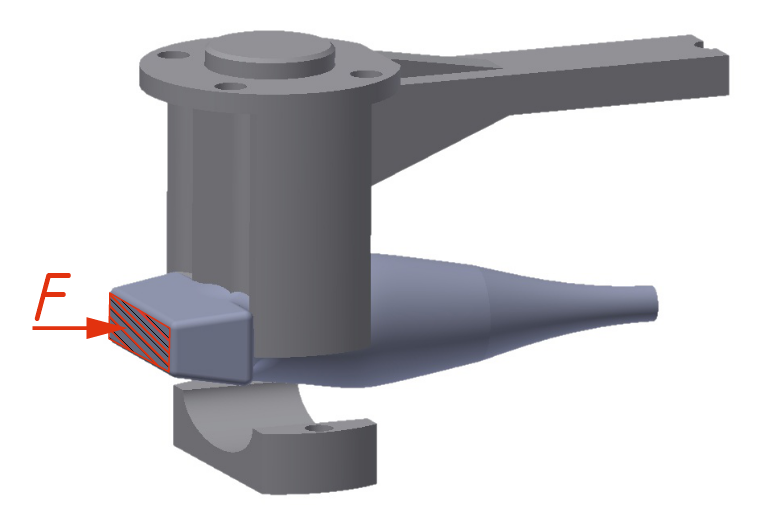
\includegraphics[width=\textwidth, keepaspectratio]{сила1адапт}
\end{minipage}
%\hfill
\begin{minipage}[h]{0.45\linewidth}
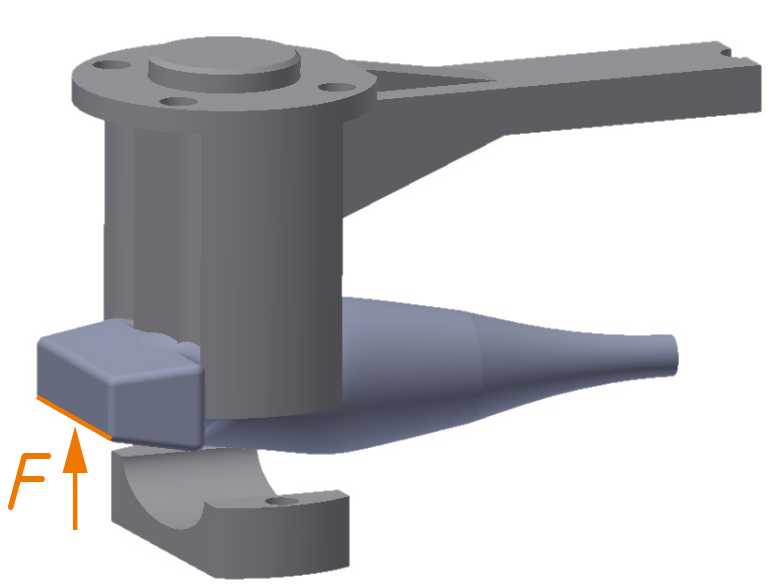
\includegraphics[width=\textwidth, keepaspectratio]{сила2адапт}
\end{minipage}
\caption{\centering \onehalfspacing {Типы нагрузок на УЗ-датчик}}
\label{risB}
\end{center}
\end{figure}

Первая нагрузка обусловлена действием силы реакции опоры со стороны тела пациента и распределена по выделенной поверхности датчика, вторая - неровностями поверхности тела, приложена к боковому ребру датчика (рисунок 2.7). Макет адаптера рассчитан диапазон действия сил от 10 до 100 Н. Для фиксации адаптера к манипулятору UR5e смоделирована фиксирующая заделка в месте закрепления адаптера. Для всех составных частей конструкции выбран материал ПВС, предел прочности при разрыв которого составляет 55 МПа. 

\section{Общий вид роботизированного комплекса}
На рисунке 9 представлен чертеж общего вида роботизированного комплекса, в котором предполагается использовать разрабатываемую БТС.

\begin{figure}[!h]
\begin{center}
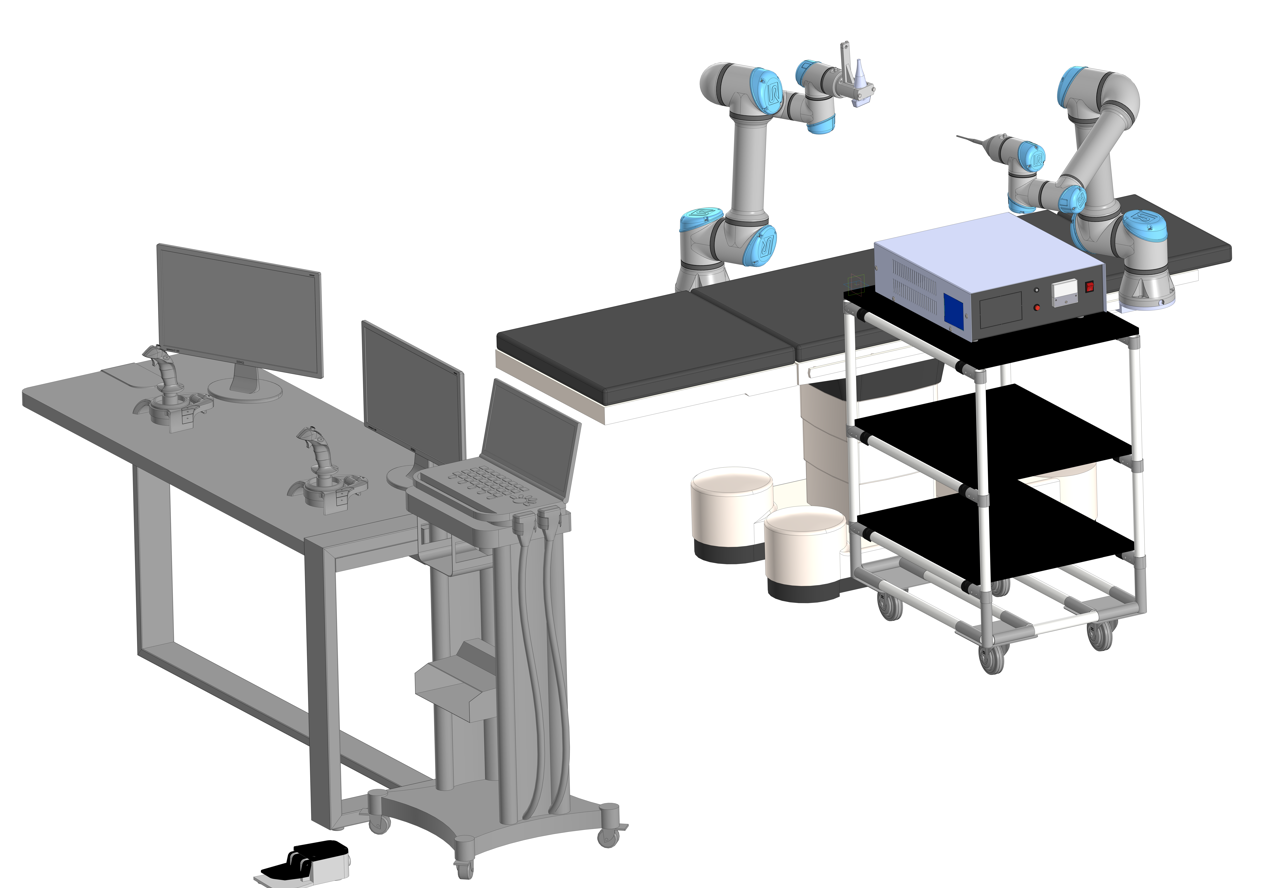
\includegraphics[width=\textwidth]{Рисунки/опер.png}
\caption{\centering \onehalfspacing {Чертеж общего вида роботизированного комплекса}}
\label{част}
\end{center}
\end{figure}

Операционный блок - специальное помещение хирургического отделения, предназначенное для выполнения операций и проведения мероприятий по их обеспечению. Операционный блок, оснащенный роботизированной системой, включает в себя операционный стол, по бокам которого расположены визуализирующий и хирургический манипуляторы, и УЗ-аппарат.Роботы-манипуляторы перемещаются вдоль операционного стола с помощью боковых рельсов, на которых закрепляются с помощью болтов. На конечном звене визуализирующего манипулятора закреплен УЗ-датчик с помощью разработанного адаптера. На хирургическом манипуляторе закреплен ультразвуковой узел.
\section{Система передачи УЗ-изображения на ПК}
В настоящее время существуют два способа передачи данных с ультразвукового аппарата: в режиме реального времени и путем сохранения, обработки и передачи данных для анализа. При использовании технологии сохранения/передачи данных исследование проводится дистанционно, полностью автономно, все УЗ-изображения сохраняются на сканере, а потом передаются для анализа. Такая технология не подходит для решения поставленных задач, так как врачу необходимо контролировать движение инструмента в режиме реального времени \cite{litlink1}.

В режиме реального времени происходит потоковая передача видеоизображения. Такая технология передачи данных более требовательна к пропускной способности канала связи. 

Наиболее часто используемая глубина пикселя ультразвукового изображения - 8 бит \cite{litlink2,litlink3}.

Допустимое разрешение в современных ультразвуковых исследованиях варьируется от 1024×1280 \cite{litlink4,litlink5} до 1366×768 \cite{litlink6}. 

Так как УЗ-аппарат Apogee 1100 имеет разрешение 1024×768, минимальное разрешение изображения должно быть 1024×768 пикселей. Также Apogee 1100 имеет выходы VGA и HDMI для извлечения видеопотока.

Для передачи ультразвуковых изображений в реальном времени требуется минимальная скорость передачи данных около 256 Кбит/с и минимальная частота кадров около 15 кадров в секунду. С таким техническими требованиями возможно проводить исследование в реальном времени и получать УЗ-изображения допустимого качества \cite{litlink7}.

В исследовании \cite{litlink3} устанавливается необходимая минимальная частота кадров для УЗИ - 25 кадров в секунду. Чем больше кадров в секунду, тем плавнее видеопоток. 

Аpogee 1100 имеет частоту кадров 2000 кадров/c. Так как частота обновления монитора намного меньше этого значения, допустимой видеограббера является его максимальная частота 60 fps. В исследовании \cite{litlink8} считается допустимой скорость передачи данных 800 Мбит/c (0,78 Гбит/c), а в работе \cite{litlink9} 0,1 Гбит/c. Исходя из этого, выберем оптимальной скорость передачи данных 1 Гбит/c.

Таким образом, технические требования к видеограбберу для захвата видеопотока с УЗИ-аппарата и передачи на ПК:

– захват VGA/HDMI сигнала,

– частота кадров 60 fps,

– поддержка разрешения 1024×768,

– глубина цвета – от 8 бит,

– скорость передачи данных – 1 Гбит/c.

Компактный внешний фрейм-граббер (рисунок 2), способный захватывать сигналы интерфейсов DVI и VGA с частотой обновления до 60 fps. Подключается к компьютеру через Ethernet порт, обеспечивая передачу данных со скоростью 1 Гбит/c. В устройстве имеется 3.5 мм аудиовход. 

\begin{figure}[H]
\begin{minipage}[h]{0.47\linewidth}
\center{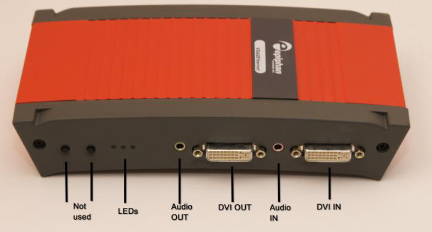
\includegraphics[width=1\linewidth]{граб1.png}} \\
\end{minipage}
\vfill
\begin{minipage}[h]{0.47\linewidth}
\center{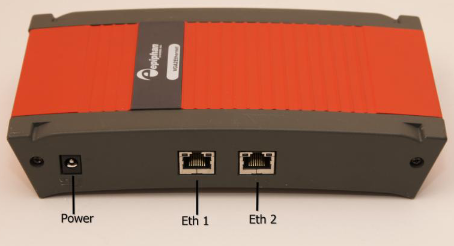
\includegraphics[width=1\linewidth]{граб11.png}} \\
\end{minipage}
\caption{Внешний вид устройства}
\label{ris:experimentalcorrelationsignals}
\end{figure}

Основные характеристики:

– поддержка интерфейсов DVI или VGA,

– частота кадров 60 fps,

– поддержка разрешений до 1920 х 1200,

– возможность работы по витой паре (Ethernet) с удаленно подключенным монитором либо проектором.

Стоимость устройства составляет 1600 долларов. 

На рисунке 3 показана схема подключения EPIPHAN VGA2Ethernet к системе.

\begin{figure}[!h]
\begin{center}
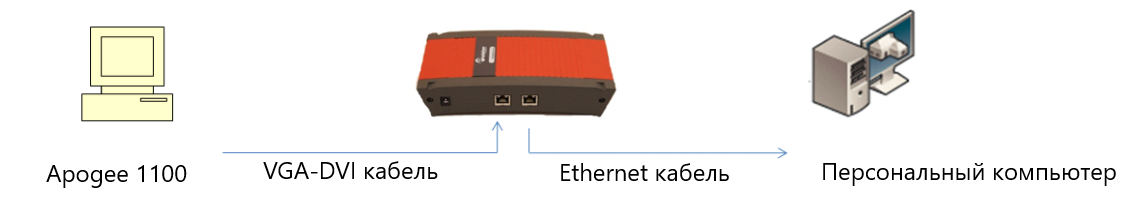
\includegraphics[width=\textwidth]{Схема граббер.png}
\caption{\centering \onehalfspacing {Схема подключения Apogee 1100 к ПК через EPIPHAN VGA2Ethernet}}
\label{част}
\end{center}
\end{figure}

Основные характеристики:

– захват изображения VGA,

– интерфейс USB 2.0,

– разрешение до 1920×1200,

– цветовое разрешение 16 бит/пиксель,

- выходной сигнал выводится c кадровой частотой от 3 до 28 Гц.

Частота обновления Epiphan VGA2USB при 1024×768 принимает значение 10 кадров в секунду. Это значение ниже допустимого порога, поэтому при использовании данного видеограббера необходимо дополнительно сжимать данные. Стоимость устройства составляет 500 долларов. 

На рисунке 4 показан внешний вид и разъемы Epiphan VGA2USB.

\begin{figure}[!h]
\begin{center}
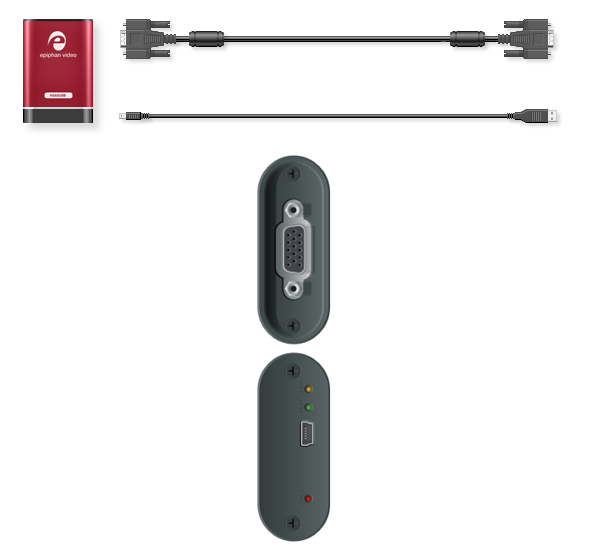
\includegraphics[width=0.6\textwidth]{граб2.png}
\caption{\centering \onehalfspacing {Внешний вид устройства}}
\label{част}
\end{center}
\end{figure}

Видеограббер позволяет выводить видеопоток с УЗ-аппарата через интерфейс VGA или DVI и передавать на ПК с помощью порта USB или Ethernet. Рассмотренные видеограбберы способны захватывать видеопоток в высоком качестве. Основным преимуществом  Epiphan VGA2USB и EPIPHAN VGA2Ethernet является то, что они поддерживают программную библиотеку для ультразвука (PLUS), которая представляет собой программный инструментарий с открытым исходным кодом для систем вмешательства под ультразвуковым контролем \cite{litlink5}. Устройства совместимы программами DirectShow и Video4Linux, что позволяет просматривать ультразвуковой видеопоток с помощью обычных видеоплееров.

\section{Решение кинематической задачи для манипулятора UR5e}

Прямая кинематическая задача заключается в расчете угла наклона конечного звена манипулятора, связанного с рабочим инструментом (УЗ-датчиком), при заданном наборе обобщенных координат остальных звеньев манипулятора.

Расположение и ориентация рабочего инструмента зависит от совместного действия вращения и/или переноса каждого сочленения цепи звеньев.  

Различают два базовых (элементарных) типа сочленений с одной степенью свободы: вращательный и поступательный. При наличии первого из них относительное расположение смежных звеньев определяется угловой переменной, при наличии второго — линейным смещением. В обоих случаях эти переменные называются обобщенными координатами:

\begin{equation}
q_{i}=\left\{\begin{array}{ll}
\theta_{i}, & \text { если звено } i \text { вращательное; } \\
d_{i}, & \text { если звено } i \text { поступательное. }
\end{array}\right.
\end{equation}

Известно, что положение и ориентация твердого тела в пространстве однозначно определяется шестью координатами: тремя линейными (декартовыми) и тремя угловыми (углами Эйлера). Использование метода Денавита-Хартенберга, позволяет сократить это число до четырех параметров, называемых параметрами Денавита-Хартенберга. Такое упрощение достигается с помощью стандартизированного алгоритма привязки систем координат к звеньям манипулятора.

Смысл введения локальных систем координат состоит в том, что поворот звена удобно выразить через поворот локальной системы координат относительно базовой, так как управление манипулятором фактически заключается в указании каждому звену обобщённых координат. Чтобы определить положение и ориентацию конечного звена, следует вычислить набор углов между сочленениями, которые приводят к соответствующей позиции рабочего инструмента. Как следствие, позиция рабочего инструмента манипулятора описывается не только в декартовых координатах, но также и в обобщённых.

Метод Денавита-Хартенберга состоит в формировании однородной матрицы преобразования, имеющей размерность 4х4 и описывающей положение системы координат каждого звена относительно системы координат предыдущего \cite{litlink10}. Это даёт возможность последовательно преобразовать координаты рабочего инструмента манипулятора из системы отсчёта, связанной с последним звеном, в базовую систему отсчёта.

Так как управление состоит в указании угла между двумя соседними звеньями – изменение этого угла приводит к изменению положения одной локальной системы координат относительно другой, что приводит к необходимости описывать каждую последующую локальную систему относительно предыдущей. Для описания изменения положения и ориентации одной локальной системы координат относительно предыдущей используются однородные матрицы преобразования.

Для описания геометрии робота-манипулятора UR5e (рисунок 5а) используется кинематическая схема, которая представляет собой графическое изображение последовательности звеньев манипулятора, соединенных между собой сочленениями (рисунок 5б).

\begin{figure}[H]
\begin{minipage}[h]{0.47\linewidth}
\center{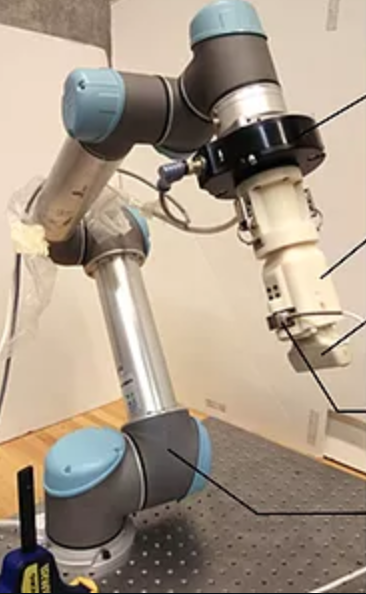
\includegraphics[width=0.5\linewidth]{сдатчиком.png}} \\a) 
\end{minipage}
\hfill
\begin{minipage}[h]{0.47\linewidth}
\center{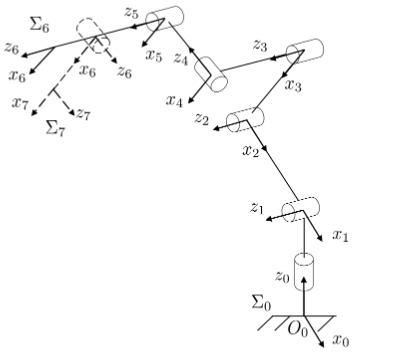
\includegraphics[width=0.9\linewidth]{кинематика1.png}} \\б)
\end{minipage}
\caption{Геометрия робота UR5e: а - робот-манипулятор с закрепленным датчиком, б - кинематическая схема (7-е звено принадлежит рабочему инструменту)}
\label{ris:experimentalcorrelationsignals}
\end{figure}

Представление Денавита-Хартенберга твёрдых звеньев зависит от четырёх геометрических параметров, соответствующих каждому звену. Эти четыре параметра полностью описывают любое вращательное или поступательное движение. Этот набор параметров достаточен для описания кинематической схемы каждого звена.

Кроме базовой системы координат для каждого звена на оси его сочленения определяется ортонормированная декартова система координат ($x_i$, $y_i$, $z_i$) , где $i=1..n$, а n равно числу степеней свободы
манипулятора (рисунок 6)\cite{litlink11}. 


\begin{figure}[!h]
\begin{center}
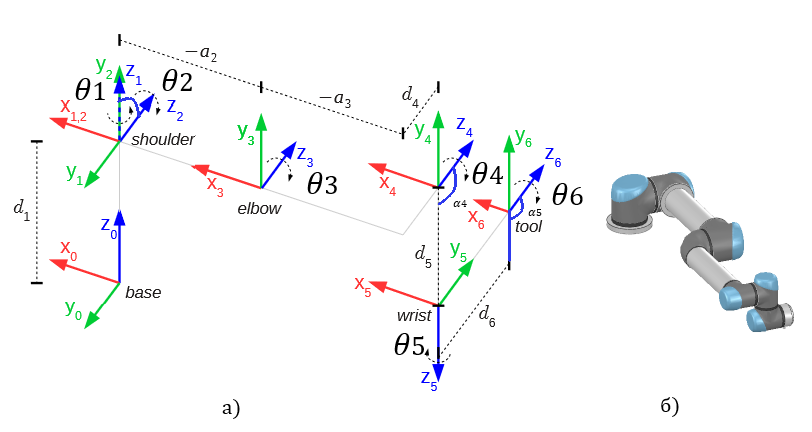
\includegraphics[width=1\textwidth]{кинематика2.png}
\caption{\centering \onehalfspacing {Определение параметров Денавита-Хартенберга: а - кинематическая схема с параметрами, б - визуализация на UR5e}}
\label{БТС}
\end{center}
\end{figure}

Поскольку вращательное сочленение имеет только одну степень свободы, каждая система координат ($x_i$, $y_i$, $z_i$) манипулятора соответствует $(i+1)$ сочленению и связана с $i$ звеном. Когда силовой привод возбуждает движение в $i$ сочленении, $i$ звено начинает двигаться относительно $(i-1)$ звена. Поскольку $i$  система координат связана с $i$  звеном, она движется вместе с ним. Таким образом, n-я система координат движется вместе с последним n-м звеном манипулятора.

$\boldsymbol{a}_{\boldsymbol{i}}$ - расстояние вдоль оси $x_{i}$ от $z_{i-1}$ до $z_{i}$;

$\boldsymbol{\alpha}_{\boldsymbol{i}}$ - угол вокруг оси $x_{i}$ от $z_{i-1}$ до $z_{i}$;

$\boldsymbol{d}_{\boldsymbol{i}}$ -  расстояние вдоль оси $z_{i-1}$ от $x_{i-1}$ до $x_{i}$;

$\boldsymbol{\theta}_{\boldsymbol{i}}$ - угол вокруг оси $z_{i-1}$ от $x_{i-1}$ до $x_{i}$.

Из четырёх параметров ($\boldsymbol{\theta}_{\boldsymbol{i}}, \boldsymbol{d}_{\boldsymbol{i}}, \boldsymbol{a}_{\boldsymbol{i}}, \boldsymbol{\alpha}_{\boldsymbol{i}}$) два параметра $\boldsymbol{\alpha}_{\boldsymbol{i}}$ и $\boldsymbol{a}_{\boldsymbol{i}}$  всегда  постоянны и  определяются  конструкцией  робота.  Один  из  двух  других параметров ($\boldsymbol{\theta}_{\boldsymbol{i}}$ либо $\boldsymbol{d}_{\boldsymbol{i}}$)  является  переменным.  Для вращательного  сочленения  величина $\boldsymbol{\theta}_{\boldsymbol{i}}$ характеризует  угол  относительного  поворота  звеньев  $i-1$  и  $i$,  а  линейная  величина $\boldsymbol{d}_{\boldsymbol{i}}$ постоянна. 

При решении прямой задачи рассматриваются две системы координат: исходная (базовая), связанная с «землей»,
$o_{0} x_{0} y_{0} z_{0}$ и итоговая $o_{n} x_{n} y_{n} z_{n}$, связанная с рабочим инструментом.

Рассмотрим подробнее два набора координат $k_{0}$ и $k_{n}$ одной и той же точки в пространстве, выраженные относительно систем $o_{0} x_{0} y_{0} z_{0}$ и $o_{n} x_{n} y_{n} z_{n}$, соответственно:

\begin{equation}
k^{0}=T_{n}^{0} k^{n},
\end{equation}

где $T_{n}^{0}$ - преобразование, несущее информацию о линейном смещении и пространственной ориентации одной системы относительно другой.

Когда системы координат сформированы для всех звеньев, можно построить однородные матрицы преобразования, связывающие i-ю и i-1-ю системы координат \cite{litlink10}:

\begin{equation}
A_{i}=\left[\begin{array}{cccc}
\operatorname{Cos} \theta_{i} & -\operatorname{Sin} \theta_{i} \operatorname{Cos} \alpha_{i} & \operatorname{Sin} \theta_{i} \operatorname{Sin} \alpha_{i} & \alpha_{i} \operatorname{Cos} \theta_{i} \\
\operatorname{Sin} \theta_{i} & \operatorname{Cos} \theta_{i} \operatorname{Cos} \alpha_{i} & -\operatorname{Cos} \theta_{i} \operatorname{Sin} \alpha_{i} & \alpha_{i} \operatorname{Sin} \theta_{i} \\
0 & \operatorname{Sin} \alpha_{i} & \operatorname{Cos} \alpha_{i} & d_{i} \\
0 & 0 & 0 & 1
\end{array}\right]
\end{equation}

Для того, чтобы получить координаты последней, шестой локальной системы координат относительно базовой необходимо провести последовательно цепочку преобразований локальных систем. Таким образом, кинематическое положение рабочего инструмента может быть получено последовательным преобразованием координат точки $R_{i} (r_{xi}, r_{yi}, r_{zi})$ из одной системы координат $i$ в другую систему координат $i-1$ следующим образом:

\begin{equation}
\begin{aligned}
&R_0=A_1*R_1, \\
&R_1=A_2*R_2, \\
&R_2=A_3*R_3, \\
&R_3=A_4*R_4, \\
&R_4=A_5*R_5, \\
&R_5=A_6*R_6.
\end{aligned}
\end{equation}

Получим:

\begin{equation}
R_0=A_1*A_2*A_3*A_4*A_5*A_6*R_6,
\end{equation}

где $A_1*A_2*A_3*A_4*A_5*A_6 = T_{6}$.

Произведение матриц преобразования также даёт матрицу преобразования, поэтому матрица $T_6$ в итоге является матрицей А и имеет такую же структуру. Матрицу $T$ называют однородной матрицей композиции преобразования. В матрице $T$ вектор $p$ является координатой центра рабочего инструмента – вектор положения, а единичные векторы, определяющие ориентацию рабочего инструмента в базовой системе называются соответственно векторами подхода – $a$, ориентации – $o$, и нормали – $n$, все они образуют правостороннюю систему координат (рисунок 7) \cite{litlink12}.

\begin{figure}[!h]
\begin{center}
\begin{minipage}[h]{0.4\linewidth}
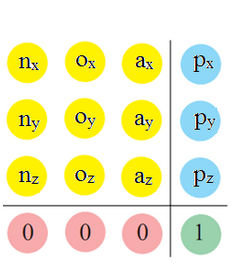
\includegraphics[width=\textwidth, keepaspectratio]{матрица.png}
\end{minipage}
%\hfill
\begin{minipage}[h]{0.4\linewidth}
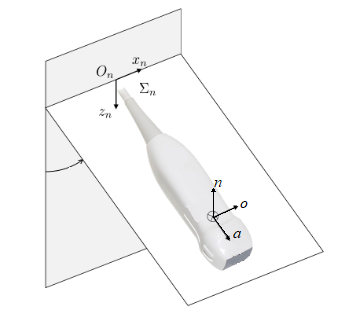
\includegraphics[width=\textwidth, keepaspectratio]{оси.png}
\end{minipage}
\caption{\centering \onehalfspacing {Структура матрицы $T_6$ и единичные векторы, определяющие ориентацию рабочего инструмента, желтым выделена матрица вращения, а синим - координаты центра рабочего инструмента}}
\label{risB}
\end{center}
\end{figure}

Так как каждый из этих векторов может быть получен в результате векторного произведения двух других, то для однозначного неизбыточного определения ориентации в пространстве достаточно выбрать любые два вектора из этой тройки.

В таблице 3.1 указаны параметры Денавита-Хартенберга для используемого робота UR5e \cite{litlink13}. Зная 6 матриц для каждого звена и, рассчитав с их помощью результирующую матрицу $T_{6}$, можно определить положение рабочего инструмента в пространстве.

\begin{table}[h]
\captionsetup[table]{singlelinecheck=false,justification=raggedleft}
\ttabbox
{\caption {\onehalfspacing Параметры Денавита-Хартенберга для робота UR5e}}
{\begin{tabular}{| >{\centering\arraybackslash}m{1.1in} | >{\centering\arraybackslash}m{1.1in} | >{\centering\arraybackslash}m{1.2in} | >{\centering\arraybackslash}m{1.2in}| >{\centering\arraybackslash}m{1.1in}|}
\hline 
Номер звена & $\boldsymbol{\theta_\boldsymbol{i}}$, рад & $\boldsymbol{a}_{\boldsymbol{i}}$, м & $\boldsymbol{d}_{\boldsymbol{i}}$, м & $\boldsymbol{\alpha}_{\boldsymbol{i}}$, рад \\ 
\hline
1 & $\boldsymbol{\theta_\boldsymbol{1}}$ & 0 & 0,1625 & $\pi/2$ \\
\hline
2 & $\boldsymbol{\theta_\boldsymbol{2}}$ & -0,4250 & 0 & 0 \\
\hline
3 & $\boldsymbol{\theta_\boldsymbol{3}}$ & -0,3922 & 0 & 0 \\
\hline
4 & $\boldsymbol{\theta_\boldsymbol{4}}$ & 0 & 0,1333 & $\pi/2$ \\
\hline
5 & $\boldsymbol{\theta_\boldsymbol{5}}$ & 0 & 0,0997 & $-\pi/2$ \\
\hline
6 & $\boldsymbol{\theta_\boldsymbol{6}}$ & 0 & 0,0996 & 0 \\
\hline
\end{tabular}}
\end{table}

Обратная задача кинематики заключается в расчете обобщенных координат при заданных линейных и угловых координатах рабочего инструмента манипулятора. Эта задача является более сложной, чем прямая, поскольку имеет 8 решений для манипулятора с 6 степенями свободны, т.е. одному и тому же положению рабочего инструмента в пространстве могут соответствовать разные конфигурации робота. 

Исходными данными являются параметры Денавита-Хартенберга и матрица $T_{6}$. Матрица вращения находится из $T_{6}$ (выделена желтым на рисунке 7) и имеет вид:

\begin{equation}
R_{n}^{0}(q)=\left[\begin{array}{lll}
r_{11}(q) & r_{12}(q) & r_{13}(q) \\
r_{21}(q) & r_{22}(q) & r_{23}(q) \\
r_{31}(q) & r_{32}(q) & r_{33}(q) 
\end{array}\right].
\end{equation}

Используя эти данные, находим $\theta$ для звена 1,5,6 \cite{litlink14}:

\begin{equation}
\theta_{1}=& \operatorname{arctg}\left(p_{y}-d_{6} r_{23}, p_{x}-d_{6} r_{13}\right)+\frac{\pi}{2} \\
& \pm \arccos \left(\frac{d_{4}}{\sqrt{\left(p_{y}-d_{6} r_{23}\right)^{2}+\left(p_{x}-d_{6} r_{13}\right)^{2}}}\right),
\end{equation}

\begin{equation}
\theta_{5}=\pm \arccos \left(\frac{p_{x}\operatorname{sin} \theta_{1}-p_{y}\operatorname{cos} \theta_{1}-d_{4}}{d_{6}}\right),
\end{equation}

\begin{equation}
\theta_{6}=\operatorname{arctg}\left(\frac{\operatorname{cos} \theta_{1} r_{22}-\operatorname{sin} \theta_{1} r_{12}}{\operatorname{sin} \theta_{5}}, \frac{\operatorname{sin} \theta_{1} r_{11}-\operatorname{cos}\theta_{1} r_{21}}{\operatorname{sin} \theta_{5}}\right).
\end{equation}
\\

Для нахождения $\theta_\boldsymbol{2}$, $\theta_\boldsymbol{3}$ и $\theta_\boldsymbol{4}$ рассчитаем $A_{3}$, $B_{3}$, $A_{4}$, $B_{4}$, $C_{4}$ и $D_{4}$:

\begin{equation}
\begin{aligned}
A_{3}=d_{5} \operatorname{sin} \theta_{6}\left(\operatorname{cos} \theta_{1} r_{11}+\operatorname{sin} \theta_{1} r_{21}\right)+d_{5} \operatorname{cos} \theta_{6}\left(\operatorname{cos} \theta_{1} r_{12}+\operatorname{sin} \theta_{1} r_{22}\right)\\-d_{6}\left(\operatorname{cos} \theta_{1} r_{13}+\operatorname{sin} \theta_{1} r_{23}\right)+p_{x} \operatorname{cos} \theta_{1}+p_{y} \operatorname{sin} \theta_{1},
\end{aligned}
\end{equation}

\begin{equation}
B_{3}=d_{5}\left(\operatorname{sin} \theta_{6} r_{31}+\operatorname{cos} \theta_{6} r_{32}\right)-d_{6} r_{33}+p_{z}-d_{1}.
\end{equation}

\begin{equation}
\begin{aligned}
&A_{4}=\operatorname{cos} \theta_{1} r_{11}+\operatorname{sin} \theta_{1} r_{21}, \\
&B_{4}=\operatorname{cos} \theta_{1} r_{12}+\operatorname{sin} \theta_{1} r_{22}, \\
&C_{4}=\operatorname{cos} \theta_{1} r_{13}+\operatorname{sin} \theta_{1} r_{23}, \\
&D_{4}=\operatorname{cos} \theta_{6} r_{31}-\operatorname{sin} \theta_{6} r_{32}.
\end{aligned}
\end{equation}

Тогда:

\begin{equation}
\theta_{3}=\pm \arccos \left(\frac{A_{3}^{2}+B_{3}^{2}-a_{2}^{2}-a_{3}^{2}}{2 a_{2} a_{3}}\right),
\end{equation}

\begin{equation}
\theta_{2}=\arcsin \left(\frac{-\operatorname{sin} \theta_{3} a_{3}}{\sqrt{A_{3}^{2}+B_{3}^{2}}}\right)+\operatorname{arctg}\left(B_{3}, A_{3}\right),
\end{equation}

\begin{equation}
\begin{aligned}
\operatorname{cos} \theta_{4}=\operatorname{cos}\left(\theta_{3}+\theta_{2}\right)\left(\operatorname{cos}\theta_{5} \operatorname{cos}\theta_{6} A_{4}-\operatorname{cos}\theta_{5} \operatorname{sin}\theta_{6} B_{4}-\operatorname{sin}\theta_{5} C_{4}\right)\\ + \operatorname{sin}\left(\theta_{3}+\theta_{2}\right)\left(\operatorname{cos} \theta_{5} D_{4}-\operatorname{sin} \theta_{5} r_{33}\right),
\end{aligned}
\end{equation}

\begin{equation}
\begin{aligned}
\operatorname{sin}\theta_{4}=\operatorname{sin}\left(\theta_{3}+\theta_{2}\right)\left(-\operatorname{cos} \theta_{5} \operatorname{cos} \theta_{6} A_{4}+\operatorname{cos} \theta_{5} \operatorname{sin} \theta_{6}B_{4}+\operatorname{sin} \theta_{5}C_{4}\right)\\+\operatorname{cos}{\theta_{3}+\theta_{2}}\left(\operatorname{cos} \theta_{5} D_{4}-\operatorname{sin} \theta_{5} r_{33}\right),
\end{aligned}
\end{equation}


\begin{equation}
{\theta_{4}=\operatorname{arctg}\left(\operatorname{sin} \theta_{4}, \operatorname{cos} \theta_{4}\right)}.
\end{equation}



\section{Выводы к главе 2}
В ходе проектирования биотехнической системы были сформулированы техническое задание и требования к БТС, в соответствии с требованиями разработана БТС, структурная и функциональная схемы, представленные в приложении А (рисунок А.2 и рисунок А.3). В части аппаратной реализации описан алгоритм работы все составных блоков аппаратной части, сформирована элементная база с учетом выполняемых системой задач. 
